% Gráfico editável no Overleaf: origem = EXP-01J, comparacao_elegibilidade.csv.
% Limiar de decisão fixo: score > 0,50. Não ajustado para atingir 63.
\begin{figure}[htbp]
\centering
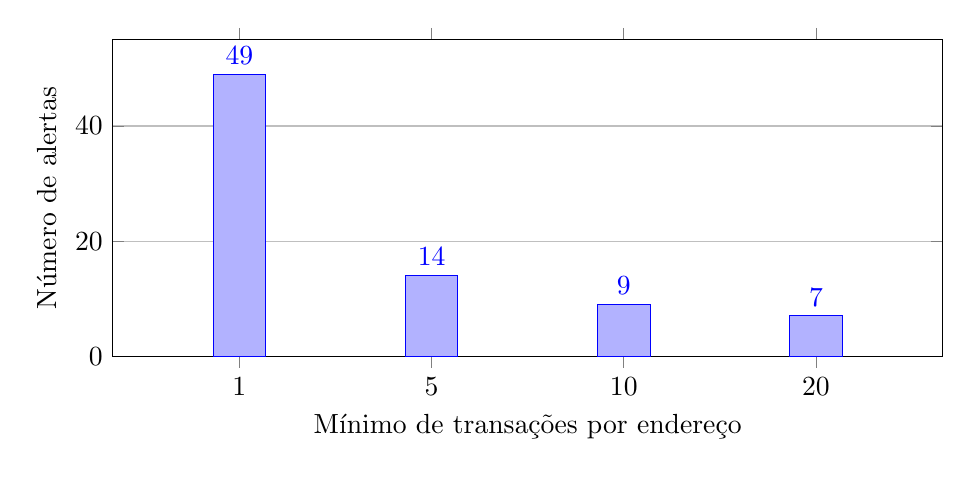
\begin{tikzpicture}
  \begin{axis}[
    ybar,
    width=\linewidth,
    height=5.6cm,
    bar width=19pt,
    ymin=0,
    ymax=55,
    ylabel={Número de alertas},
    xlabel={Mínimo de transações por endereço},
    symbolic x coords={1,5,10,20},
    xtick=data,
    nodes near coords,
    nodes near coords align={vertical},
    enlarge x limits=0.22,
    grid=major,
    ymajorgrids=true,
    xmajorgrids=false,
    ]
    \addplot coordinates {(1,49) (5,14) (10,9) (20,7)};
  \end{axis}
\end{tikzpicture}
\caption{Sensibilidade ao critério de elegibilidade no dia 29/10/2020: mesmo modelo Random Forest e limiar fixo de 0,50.}
\label{fig:sensibilidade}
\end{figure}
